\section{Desarrollo}
\subsection{Teorema de Sustitución}
Para este ejercicio se utilizó el siguiente circuito:
\begin{center}
	\begin{circuitikz}[scale=0.8] % Ajusta la escala si el circuito es muy grande
		% Definimos nodos clave (coordenadas) para guiar el dibujo
		\coordinate (A) at (0,4);
		\coordinate[label=above:a] (B) at (4,4);
		\coordinate (C) at (8,4);
		\coordinate (D) at (0,0);
		\coordinate[label=below:b] (E) at (4,0);
		\coordinate (F) at (8,0);
		
		% --- DIBUJO DEL CIRCUITO ---
		\draw (A) to[battery1, l=$E_1$] (D);
		
		\draw (A) to[R, l=$R_1$] (B);

		\draw (B) to[R, l=$R_4$] (C);
		
		\draw (C) to[R, l=$R_5$] (8,2) to[R, l=$R_6$] (F);
		
		\draw (B) to[R, l=$R_2$] (4,2) to[R, l=$R_3$] (E);
		
		\draw (D) -- (F);
	\end{circuitikz}
\end{center}
Con los valores de los componentes definidos para la experimentación:
\begin{equation*}
	\begin{matrix}
		R_1 = 3.3 \text{ k}\Omega & R_2 = 1 \text{ k}\Omega & R_3 = 1 \text{ k}\Omega \\
		R_4 = 330 \Omega & R_5 = 330 \Omega   & R_6 = 330\Omega \\
		E_1 = 9 \text{ V}
	\end{matrix}
\end{equation*}
Para la validación del teorema, se seleccionó la rama conformada por el arreglo en serie de $R_2$ y $R_3$. De acuerdo con la teoría, si la red eléctrica tiene una solución única, dicha rama puede sustituirse por una fuente ideal sin afectar las variables del resto del circuito.

\subsubsection{Parte experimental}

\begin{enumerate}
	\item Se armó el circuito original y se midieron con el multímetro digital el voltaje ($\hat{v}$) en la rama de carga (nodos 'a' a 'b').
	\begin{figure}[H]
		\centering
		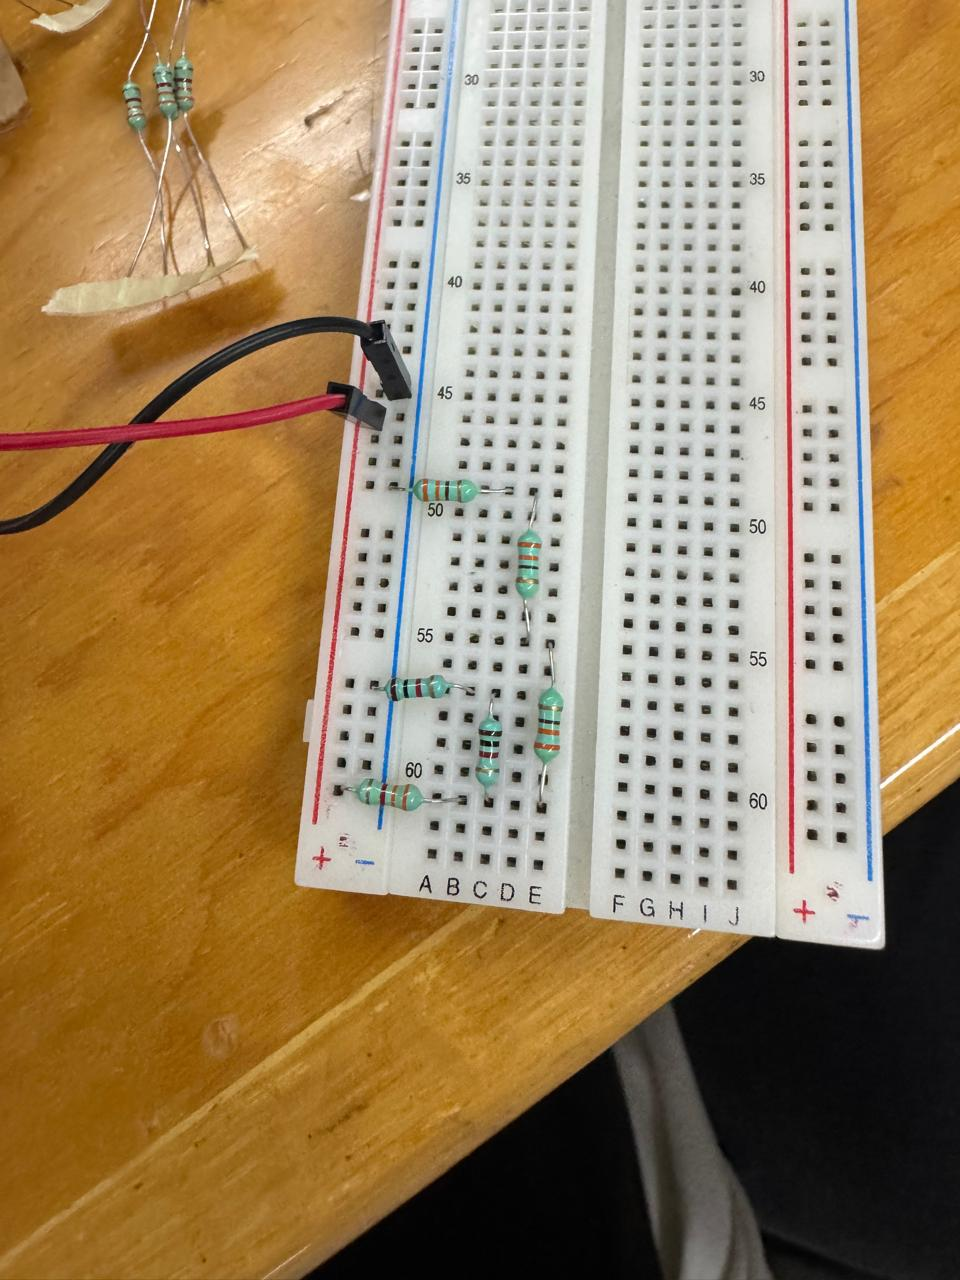
\includegraphics[width=0.4\linewidth]{assets/img/Tsustitucion_parte1.jpeg}
		\caption{Montaje experimental del circuito de 6 resistencias para el Teorema de Sustitución.}
		\label{fig:sustitucion_p1}
	\end{figure}
	\item Se procedió a retirar las resistencias $R_2$ y $R_3$, sustituyéndolas por una fuente de voltaje ajustada exactamente al valor $\hat{v}$ medido previamente.
	\begin{figure}[H]
		\centering
		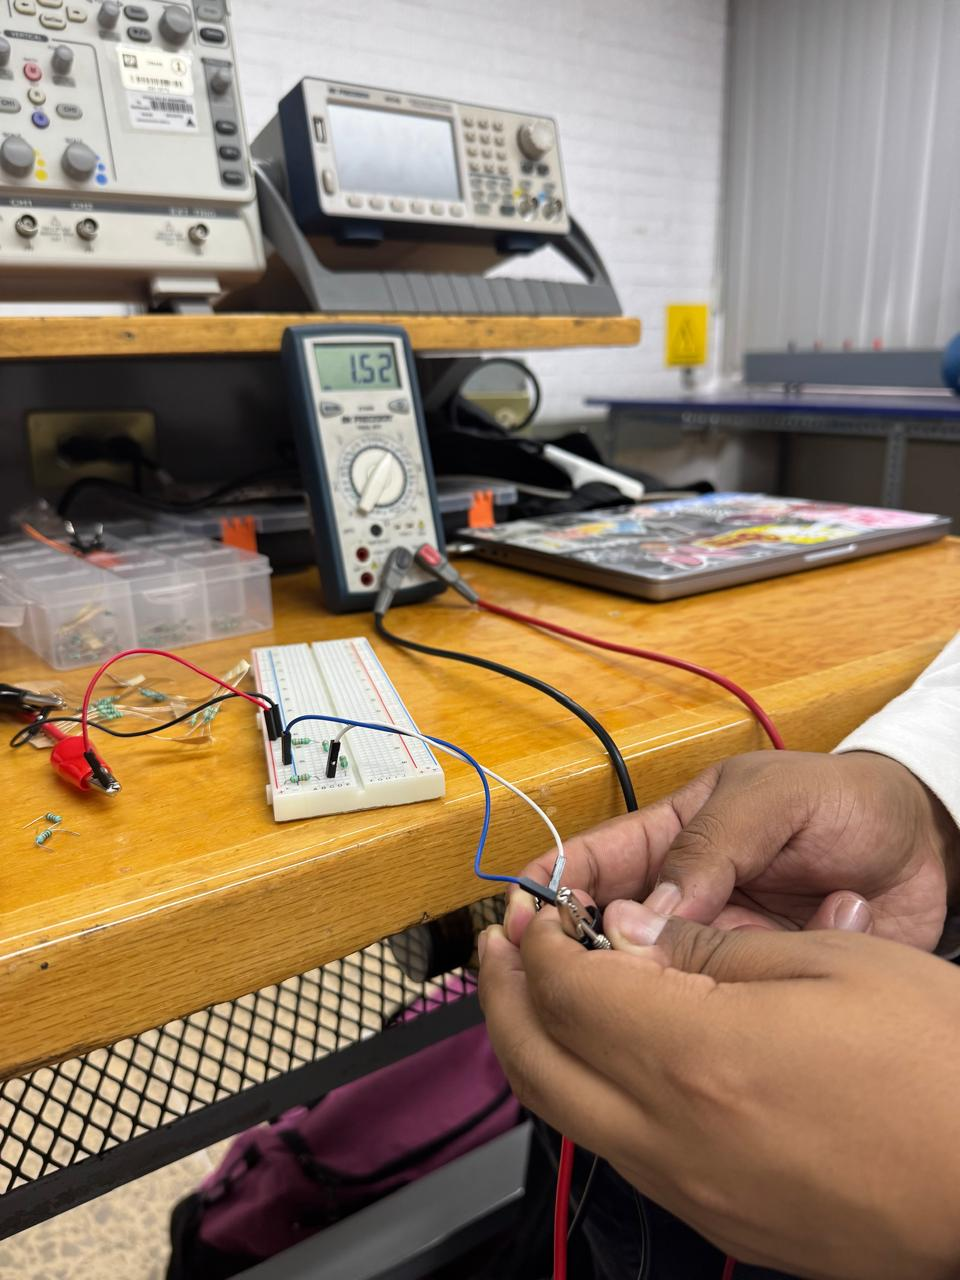
\includegraphics[width=0.4\linewidth]{assets/img/Tsustitucion_parte2.jpeg}
		\caption{Sustitución de la rama por una fuente de poder equivalente.}
		\label{fig:sustitucion_p2}
	\end{figure}
	\item Se midieron las tensiones en las resistencias restantes ($R_1$ a $R_6$) para constatar que los valores permanecieran inalterados respecto a la red original.
	\begin{figure}[H]
		\centering
		\begin{subfigure}{0.45\textwidth}
			\centering
			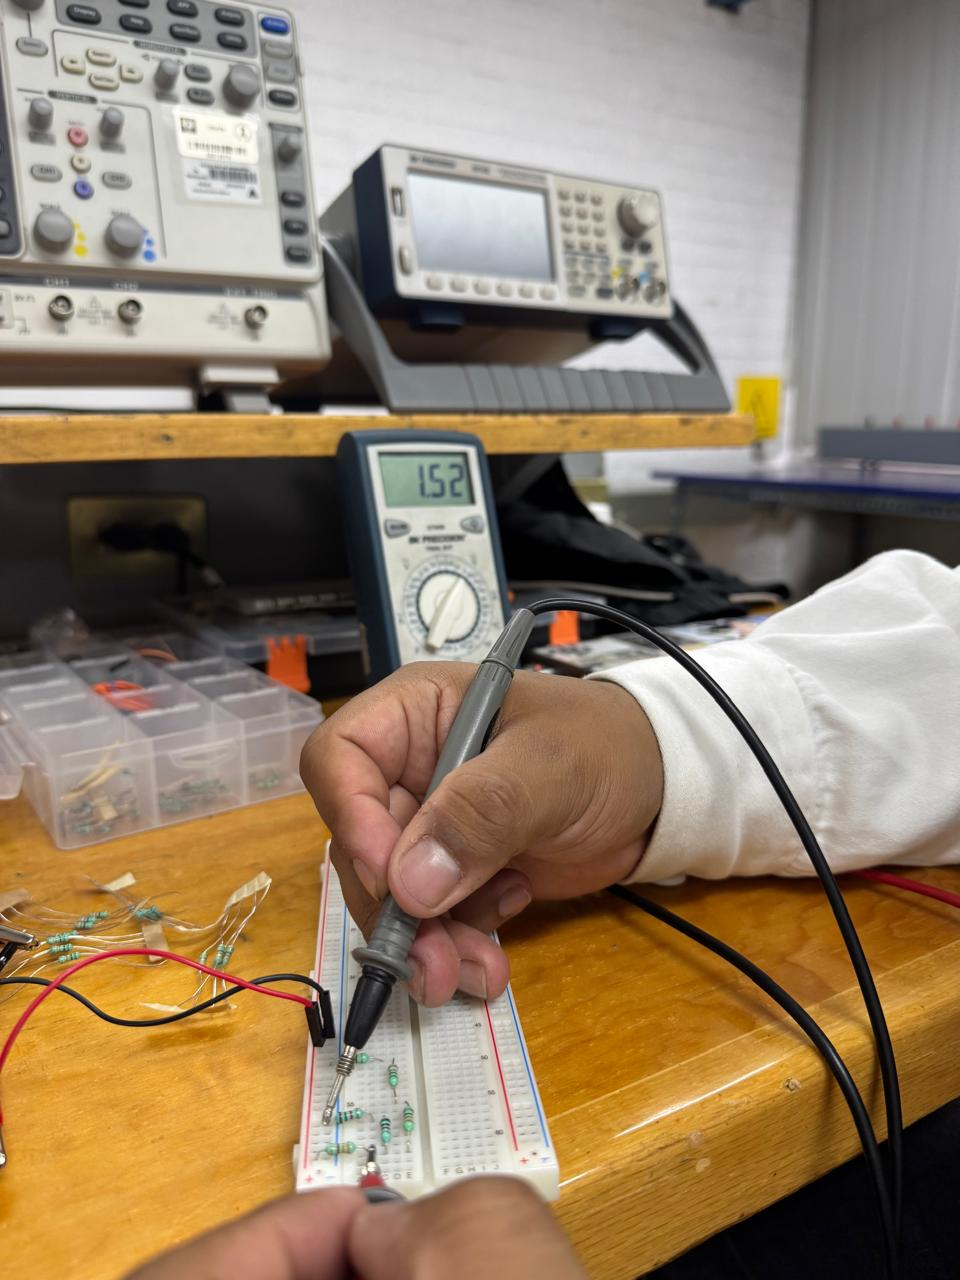
\includegraphics[width=0.8 \linewidth]{assets/img/Tsustitucion_medicion1.jpeg}
			\label{fig:sustitucion_m1}
		\end{subfigure}
		\begin{subfigure}{0.45\textwidth}
			\centering
			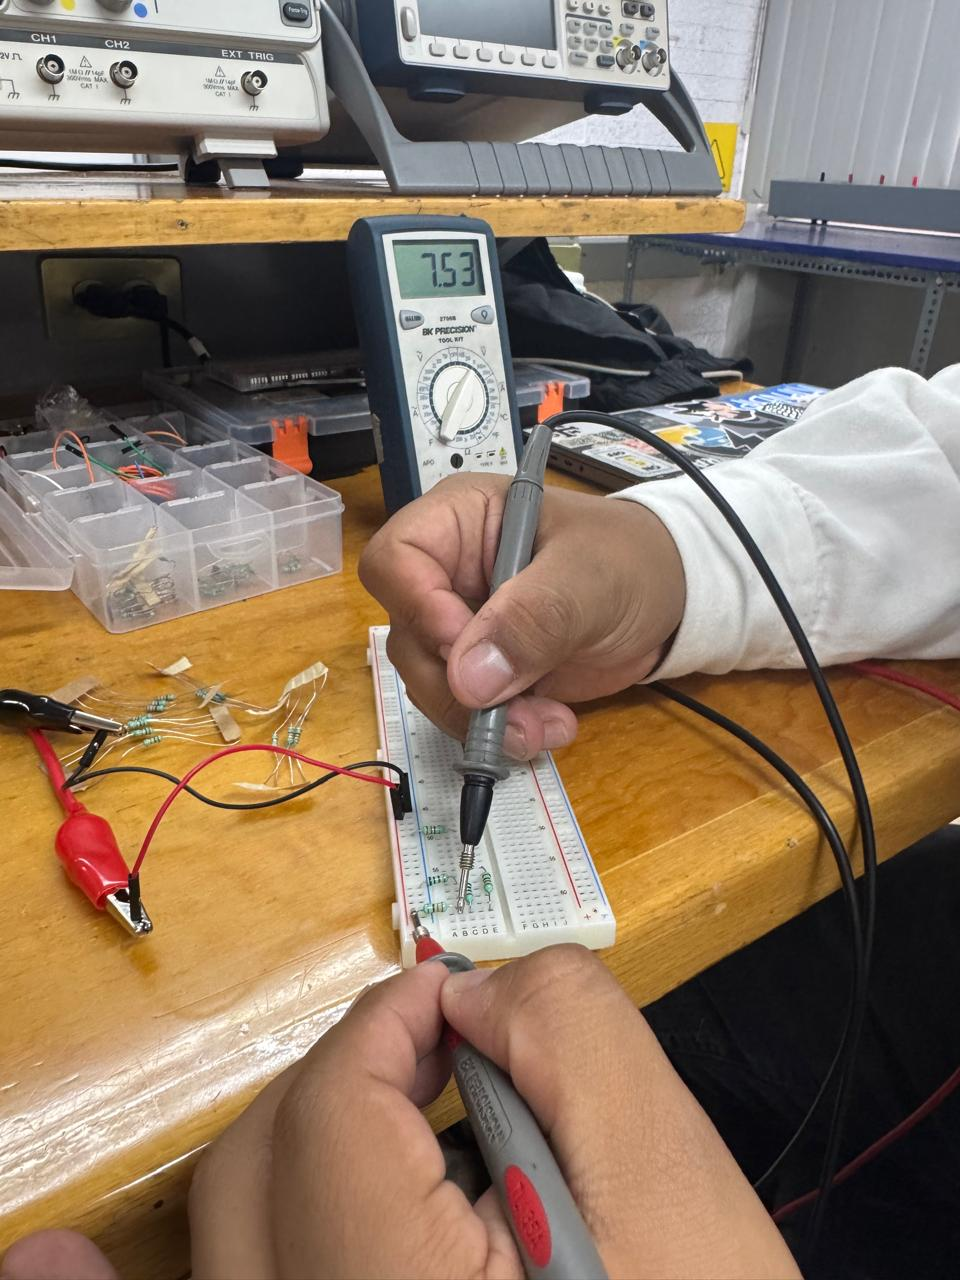
\includegraphics[width=0.8\linewidth]{assets/img/Tsustitucion_medicion2.jpeg}
			\label{fig:sustitucion_m2}
		\end{subfigure}			
		\caption{Mediciones sobre el circuito.}
	\end{figure}
\end{enumerate}

\begin{table}[H]
	\centering
	\caption{Resultados experimentales: Teorema de Sustitución.}
	\begin{tabular}{|c|c|c|c|c|c|c|}
		\hline
		\textbf{Configuración} & \textbf{$V_{E1}$ [V]} & \textbf{$V_{R1}$ [V]} & \textbf{$V_{ab}$ [V]} & \textbf{$V_{R4}$ [V]} & \textbf{$V_{R5}$ [V]} & \textbf{$V_{R6}$ [V]} \\ \hline
		Red Original & 9.05 & 7.53 & 1.52 & 0.51 & 0.51 & 0.51 \\ \hline
		Red Modificada & 9.05 & 7.53 & 1.52 & 0.51 & 0.51 & 0.51 \\ \hline
	\end{tabular}
\end{table}

Como se observa en los datos experimentales, al sustituir la rama $ab$ por una fuente de voltaje de valor idéntico a la caída de potencial original, los voltajes en las ramas adyacentes ($R_1, R_4, R_5, R_6$) no sufrieron variación alguna. Esto confirma la validez del teorema, el cual establece que la red modificada es más sencilla de analizar sin afectar las condiciones iniciales del resto de la red. 


\subsubsection{Parte teórica}

Para validar la precisión del modelo experimental, es imperativo contrastar los resultados con una referencia teórica o simulada. Esto permite establecer un margen de error y asegurar que las variaciones observadas se encuentren dentro de los límites de tolerancia de los componentes y equipos de medición. La simulación actúa como una representación ideal que fundamenta la unicidad de la solución de la red. El proceso de validación siguió la siguiente metodología:

\begin{enumerate}
	\item Implementación del esquema circuital original en el entorno de simulación para obtener los parámetros de referencia.
	
		\begin{figure}[H]
		\centering
		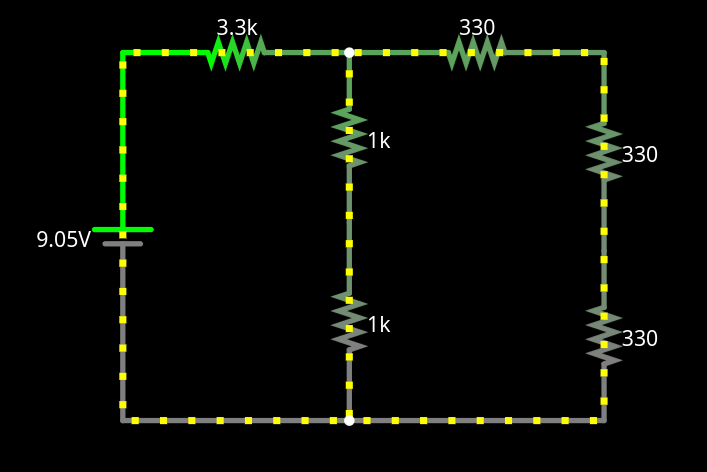
\includegraphics[width=0.4\linewidth]{assets/img/Tsustitucion_simulacion1.png}
		\caption{.}
		\label{fig:sustitucion_s1}
	\end{figure}
	
	\item Aplicación del teorema de sustitución mediante el reemplazo de la rama $ab$ por una fuente de voltaje ideal de valor equivalente a la caída de potencial obtenida.

	\begin{figure}[H]
		\centering
		\begin{subfigure}{0.45\textwidth}
			\centering
			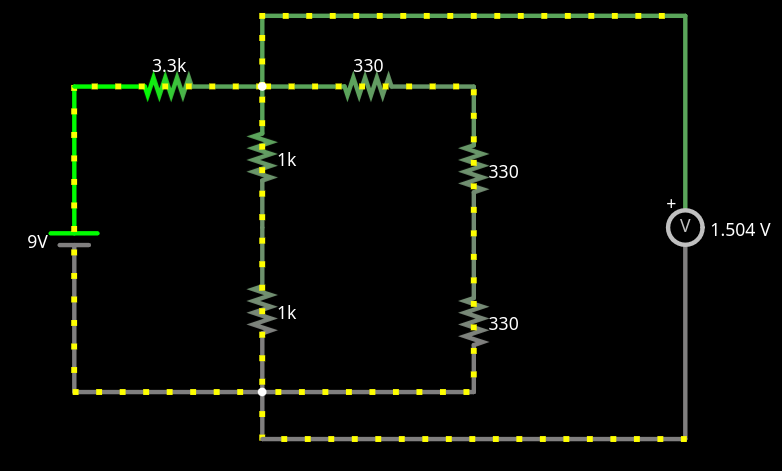
\includegraphics[width=0.8 \linewidth]{assets/img/Tsustitucion_simulacion2.png}
			\label{fig:sustitucion_s2}
		\end{subfigure}
		\begin{subfigure}{0.45\textwidth}
			\centering
			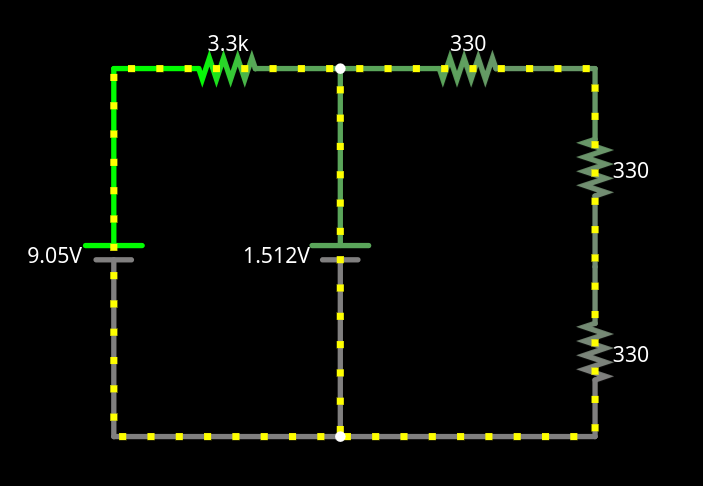
\includegraphics[width=0.8\linewidth]{assets/img/Tsustitucion_simulacion3.png}
			\label{fig:sustitucion_s3}
		\end{subfigure}			
		\caption{.}
	\end{figure}
	
	\item Verificación de la invariancia de los valores de tensión y corriente en el resto de la red tras la modificación.

	\begin{figure}[H]
		\centering
		\begin{subfigure}{0.45\textwidth}
			\centering
			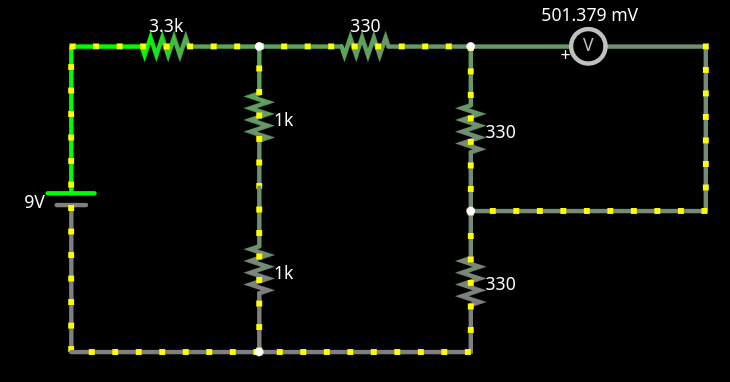
\includegraphics[width=0.8 \linewidth]{assets/img/Tsustitucion_simulacion4.png}
			\label{fig:sustitucion_s4}
		\end{subfigure}
		\begin{subfigure}{0.45\textwidth}
			\centering
			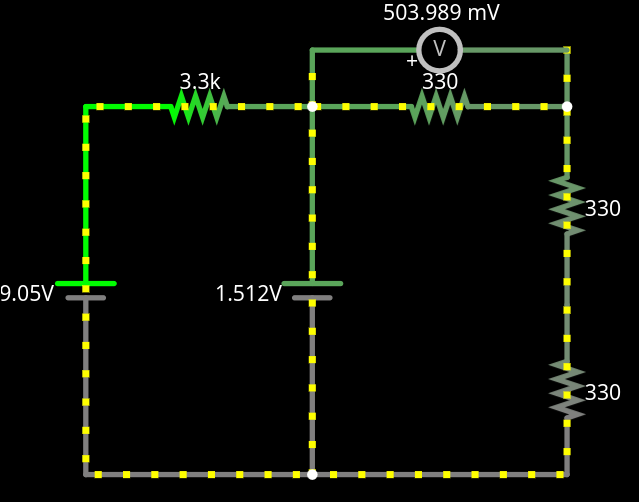
\includegraphics[width=0.8
			\linewidth]{assets/img/Tsustitucion_simulacion5.png}
			\label{fig:sustitucion_s5}
		\end{subfigure}			
		\caption{.}
	\end{figure}

\end{enumerate}

\begin{table}[h!]
	\centering
	\caption{Resultados de simulación.}
	\begin{tabular}{|c|c|c|c|c|c|c|}
		\hline
		\textbf{Configuración} & \textbf{$V_{E1}$ [V]} & \textbf{$V_{R1}$ [V]} & \textbf{$V_{ab}$ [V]} & \textbf{$V_{R4}$ [V]} & \textbf{$V_{R5}$ [V]} & \textbf{$V_{R6}$ [V]} \\ \hline
		Red Original & 9.05 & 7.537 & 1.513 & 0.504 & 0.504 & 0.504 \\ \hline
		Red Modificada & 9.05 & 7.538 & 1.512 & 0.504 & 0.504 & 0.504 \\ \hline
	\end{tabular}
\end{table}

\textbf{Análisis de la Unicidad y Leyes de Kirchhoff}

La validez del teorema de sustitución se fundamenta en la suposición de la unicidad de la solución de las redes eléctricas para un conjunto de entradas dado. Al emplear los valores obtenidos en la simulación, se observa que tanto en la red original como en la modificada se satisfacen con precisión las leyes de Kirchhoff, confirmando que la red eléctrica modificada es más sencilla de estudiar sin alterar el comportamiento de la red original.

Para la validación matemática, se analizan los dos lazos del circuito bajo ambas configuraciones:

\begin{itemize}
	\item \textbf{Lazo de entrada (LVK 1):} En la red original, la suma de las caídas de tensión coincide exactamente con la fuente de alimentación ($7.537\text{ V} + 1.513\text{ V} = 9.050\text{ V}$). En la red modificada, al realizar la sustitución por una fuente de $1.512\text{ V}$, se observa un ajuste en la resistencia $R_1$, la cual registra $7.538\text{ V}$, manteniendo el equilibrio del lazo en $9.050\text{ V}$.
	
	\item \textbf{Lazo de carga (LVK 2):} En la configuración original, la tensión de la rama central es de $1.513\text{ V}$, mientras que la suma de las caídas en la rama derecha es $V_{R4} + V_{R5} + V_{R6} = 0.504\text{ V} + 0.504\text{ V} + 0.504\text{ V} = 1.512\text{ V}$. Tras la sustitución de la rama $ab$ por una fuente ideal de $1.512\text{ V}$, la igualdad se vuelve exacta: $1.512\text{ V} = 0.504\text{ V} + 0.504\text{ V} + 0.504\text{ V}$.
\end{itemize}

La mínima diferencia de $0.001\text{ V}$ detectada en el análisis de la red original se atribuye a los algoritmos de redondeo del simulador al manejar los parámetros concentrados de las resistencias de $330~\Omega$ y $1\text{ k}\Omega$. No obstante, la invarianza de los voltajes en las ramas $R_4, R_5$ y $R_6$ al pasar de una red a otra demuestra que la rama $R_2, R_3$ puede sustituirse por una fuente ideal sin que se afecten los voltajes y corrientes dentro del circuito.

\subsection{Teorema de Tellegen}

El teorema de Tellegen es una herramienta analítica de carácter general fundamentada exclusivamente en las leyes de Kirchhoff, lo que le permite ser independiente de la naturaleza lineal o no lineal de los componentes de la red. Este teorema establece que, para cualquier red eléctrica de parámetros concentrados y determinística, la suma algebraica de las potencias instantáneas en todas las ramas es nula:

\begin{equation}
	\sum_{k=1}^{b} v_{k} j_{k} = 0
\end{equation}

En términos físicos, representa el principio de conservación de la energía, dictando que la potencia suministrada por las fuentes activas es idéntica a la potencia total disipada por los elementos pasivos del sistema.

\subsubsection{Parte experimental}

Para la validación de este principio, se emplearon los valores de tensión y corriente obtenidos en la configuración original de la red. Se calculó la potencia individual de cada elemento ($P = V \cdot I$) para verificar el balance energético total.

\textbf{Cálculos de Corriente por resistencia}
A partir de los voltajes medidos y los valores de resistencia, se determinaron las intensidades de corriente mediante la Ley de Ohm:

\begin{itemize}
	\item $I_{R1} = \frac{7.62 \text{ V}}{3300 \text{ } \Omega} = 2.310 \text{ mA}$
	\item $I_{R2} = \frac{0.76 \text{ V}}{1000 \text{ } \Omega} = 0.760 \text{ mA}$
	\item $I_{R3} = \frac{0.78 \text{ V}}{1000 \text{ } \Omega} = 0.780 \text{ mA}$
	\item $I_{R4} = \frac{0.52 \text{ V}}{330 \text{ } \Omega} = 1.576 \text{ mA}$
	\item $I_{R5} = \frac{0.52 \text{ V}}{330 \text{ } \Omega} = 1.576 \text{ mA}$
	\item $I_{R6} = \frac{0.52 \text{ V}}{330 \text{ } \Omega} = 1.576 \text{ mA}$
\end{itemize}

\textbf{Balance de Potencias}
En la Tabla \ref{tab:tellegen_mw} se desglosan los voltajes y las potencias calculadas para cada componente del circuito.

\begin{table}[h!]
	\centering
	\caption{Balance de Potencias Experimentales (mW).}
	\label{tab:tellegen_mw}
	\begin{tabular}{|l|c|c|}
		\hline
		\textbf{Elemento} & \textbf{Voltaje [V]} & \textbf{Potencia [mW]} \\ \hline
		Fuente $E_1$ & 9.08 & 20.8 \\ \hline
		Resistencia $R_1$ & 7.62 & 17.5 \\ \hline
		Resistencia $R_2$ & 0.76 & 0.578 \\ \hline
		Resistencia $R_3$ & 0.78 & 0.592 \\ \hline
		Resistencia $R_4$ & 0.52 & 0.822 \\ \hline
		Resistencia $R_5$ & 0.52 & 0.822 \\ \hline
		Resistencia $R_6$ & 0.52 & 0.822 \\ \hline
	\end{tabular}
\end{table}

\textbf{Análisis de Resultados}
La suma de las potencias absorbidas por las resistencias en la red es:
\begin{equation}
	P_{abs} = 17.5 + 0.578 + 0.592 + 0.822 + 0.822 + 0.822 = 21.136 \text{ mW}
\end{equation}

Al comparar este resultado con la potencia suministrada por la fuente ($P_{sum} = 20.8 \text{ mW}$), se observa una diferencia residual de:
\begin{equation}
	\Delta P = |21.136 - 20.800| = 0.336 \text{ mW}
\end{equation}

Esta discrepancia de aproximadamente $0.3 \text{ mW}$ es consistente con los cálculos manuales y se atribuye a los errores de redondeo en las mediciones de voltaje y a la tolerancia de los instrumentos de laboratorio. El resultado confirma experimentalmente la validez del teorema y la conservación de la energía en el sistema bajo estudio.

\subsection{Teorema de Thévenin}

El objetivo de esta fase es modelar una red lineal activa mediante un circuito equivalente simplificado (fuente de tensión en serie con una resistencia). El circuito bajo estudio presenta múltiples fuentes y una red resistiva compleja, cuya configuración se detalla a continuación:

\begin{center}
	\begin{circuitikz}[scale=0.8]
		\draw (0,4) to[battery1, l=$E_1$] (0,0);
		\draw (0,4) to[R, l=$R_1$] (3,4) to[short, -*] (9,4) node[above] {a};
		\draw (3,4) to[R, l=$R_2$] (3,0);
		\draw (5,4) to[battery1, l=$E_2$] (5,0); 
		\draw (8,4) to[R, l=$R_3$] (8,2) to[R, l=$R_4$] (8,0);
		\draw (8,2) to[short, -*] (9,2) node[below] {b};
		\draw (0,0) -- (8,0);
	\end{circuitikz}
\end{center}

	\begin{figure}[H]
	\centering
	\begin{subfigure}{0.45\textwidth}
		\centering
		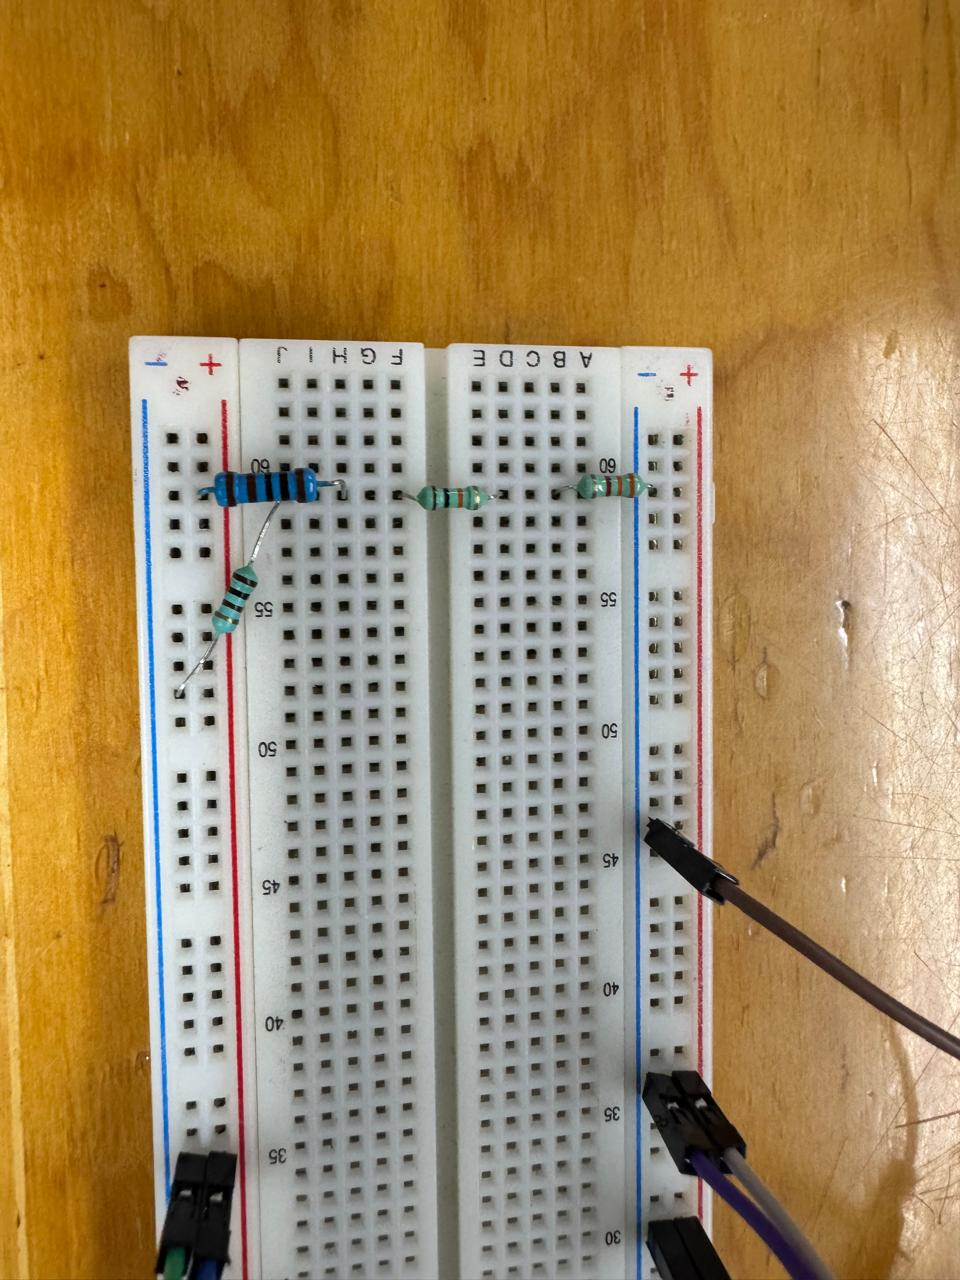
\includegraphics[width=0.8 \linewidth]{assets/img/Tthevenin_circuito1.jpeg}
		\label{fig:thevenin_s1}
	\end{subfigure}
	\begin{subfigure}{0.45\textwidth}
		\centering
		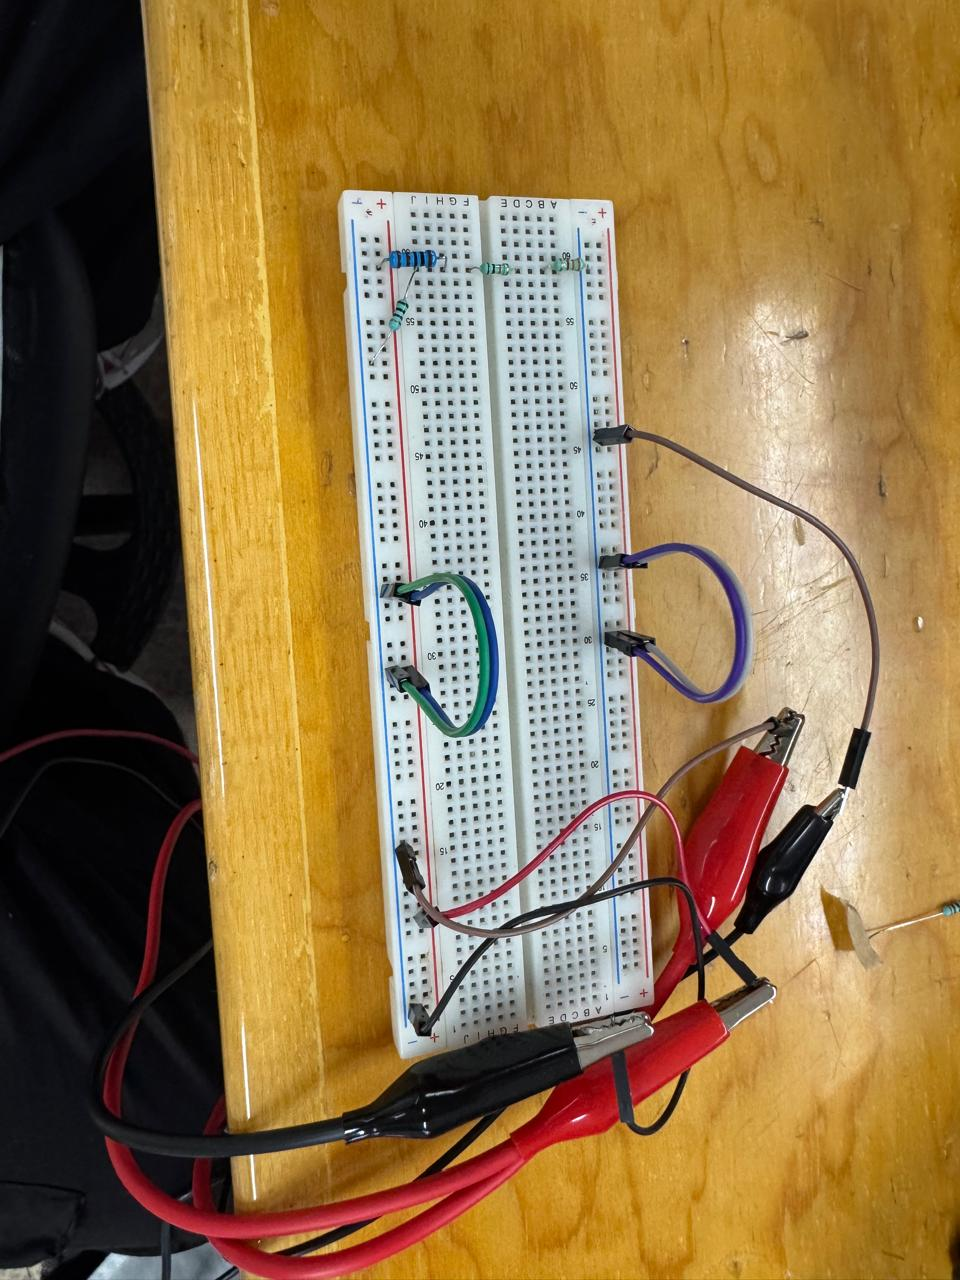
\includegraphics[width=0.8
		\linewidth]{assets/img/Tthevenin_circuito1_2.jpeg}
		\label{fig:thevenin_s2}
	\end{subfigure}			
	\caption{Circuito armado en laboratorio.}
\end{figure}

Los parámetros de los componentes para esta red activa son:
\begin{equation*}
	\begin{matrix}
		E_1 = 12.05 \text{ V} & E_2 = 6.014 \text{ V} & R_1 = 999 \text{ }\Omega \\
		R_2 = 97.2 \text{ }\Omega & R_3 = 9.62 \text{ k}\Omega & R_4 = 3.214 \text{ k}\Omega
	\end{matrix}
\end{equation*}

\subsubsection{Parte experimental}

La metodología para la validación del teorema consistió en tres etapas: la caracterización de la red, la prueba bajo carga y la validación del modelo equivalente.

\begin{enumerate}
	\item \textbf{Obtención de parámetros de Thévenin:} Se midió el voltaje de circuito abierto ($V_{th}$) entre las terminales $a$ y $b$, y posteriormente se determinó la resistencia equivalente ($R_{th}$) mediante la anulación de las fuentes independientes.
	
		\begin{figure}[H]
		\centering
		\begin{subfigure}{0.45\textwidth}
			\centering
			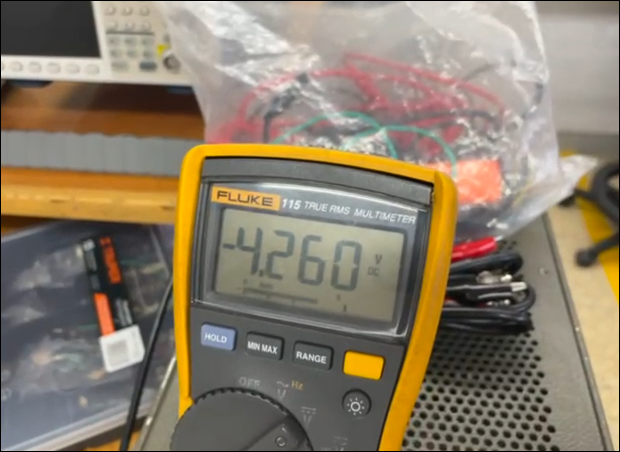
\includegraphics[width=0.8 \linewidth]{assets/img/Tthevenin_medicion1.png}
			\label{fig:thevenin_s3}
			\caption{Valor de la caída de voltaje en $ab$.}
		\end{subfigure}
		\begin{subfigure}{0.45\textwidth}
			\centering
			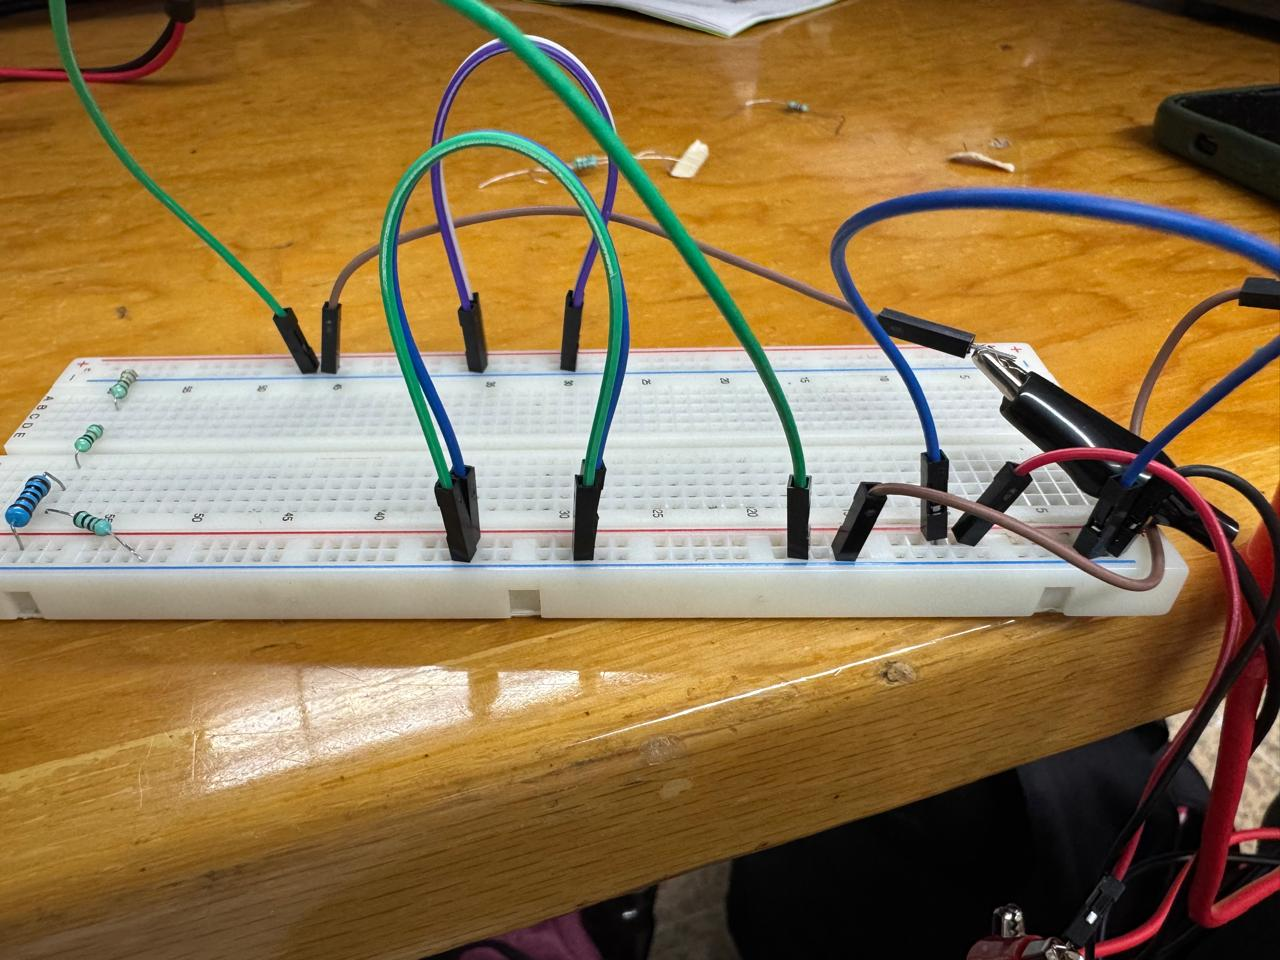
\includegraphics[width=0.8
			\linewidth]{assets/img/Tthevenin_medicion2.jpeg}
			\label{fig:thevenin_s4}
			\caption{Fuentes puenteadas para la medición de $R'$.}
		\end{subfigure}			
	\end{figure}
	
	\begin{itemize}
		\item Voltaje de Thévenin ($V_{th}$) = $-4.26 \text{ V}$
		\item Resistencia de Thévenin ($R_{th}$) = $2.424 \text{ k}\Omega$
	\end{itemize}
	
	\item \textbf{Prueba de la red activa bajo carga:} Se conectaron tres resistencias de carga ($R_L$) distintas en las terminales $a$ y $b$ de la red original, midiendo la tensión de salida para cada caso.
	
	\begin{figure}[H]
		\centering
		\begin{subfigure}{0.3\textwidth}
			\centering
			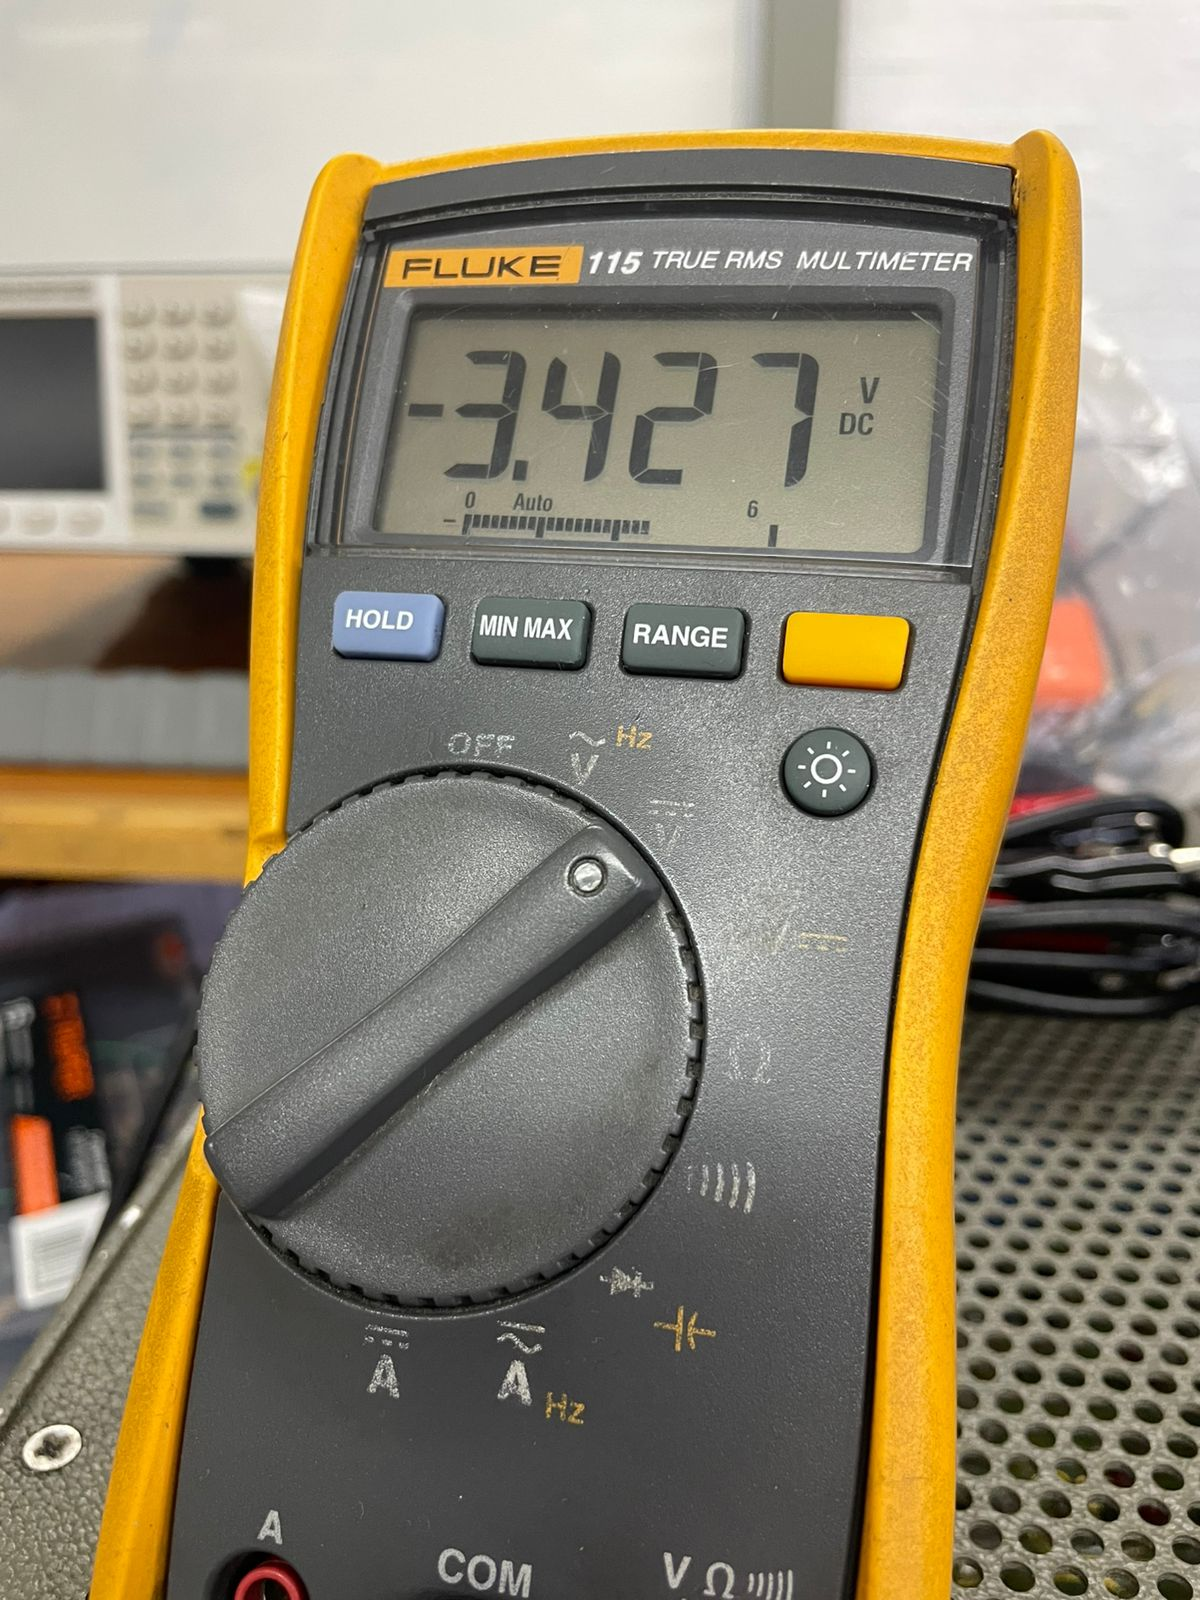
\includegraphics[width=0.8 \linewidth]{assets/img/Tthevenin_medicion3_1.jpeg}
			\label{fig:thevenin_s5}
			\caption{Valor de la caída de voltaje para $R_{ab}=9.88 \text{k}\Omega$.}
		\end{subfigure}
		\begin{subfigure}{0.3\textwidth}
			\centering
			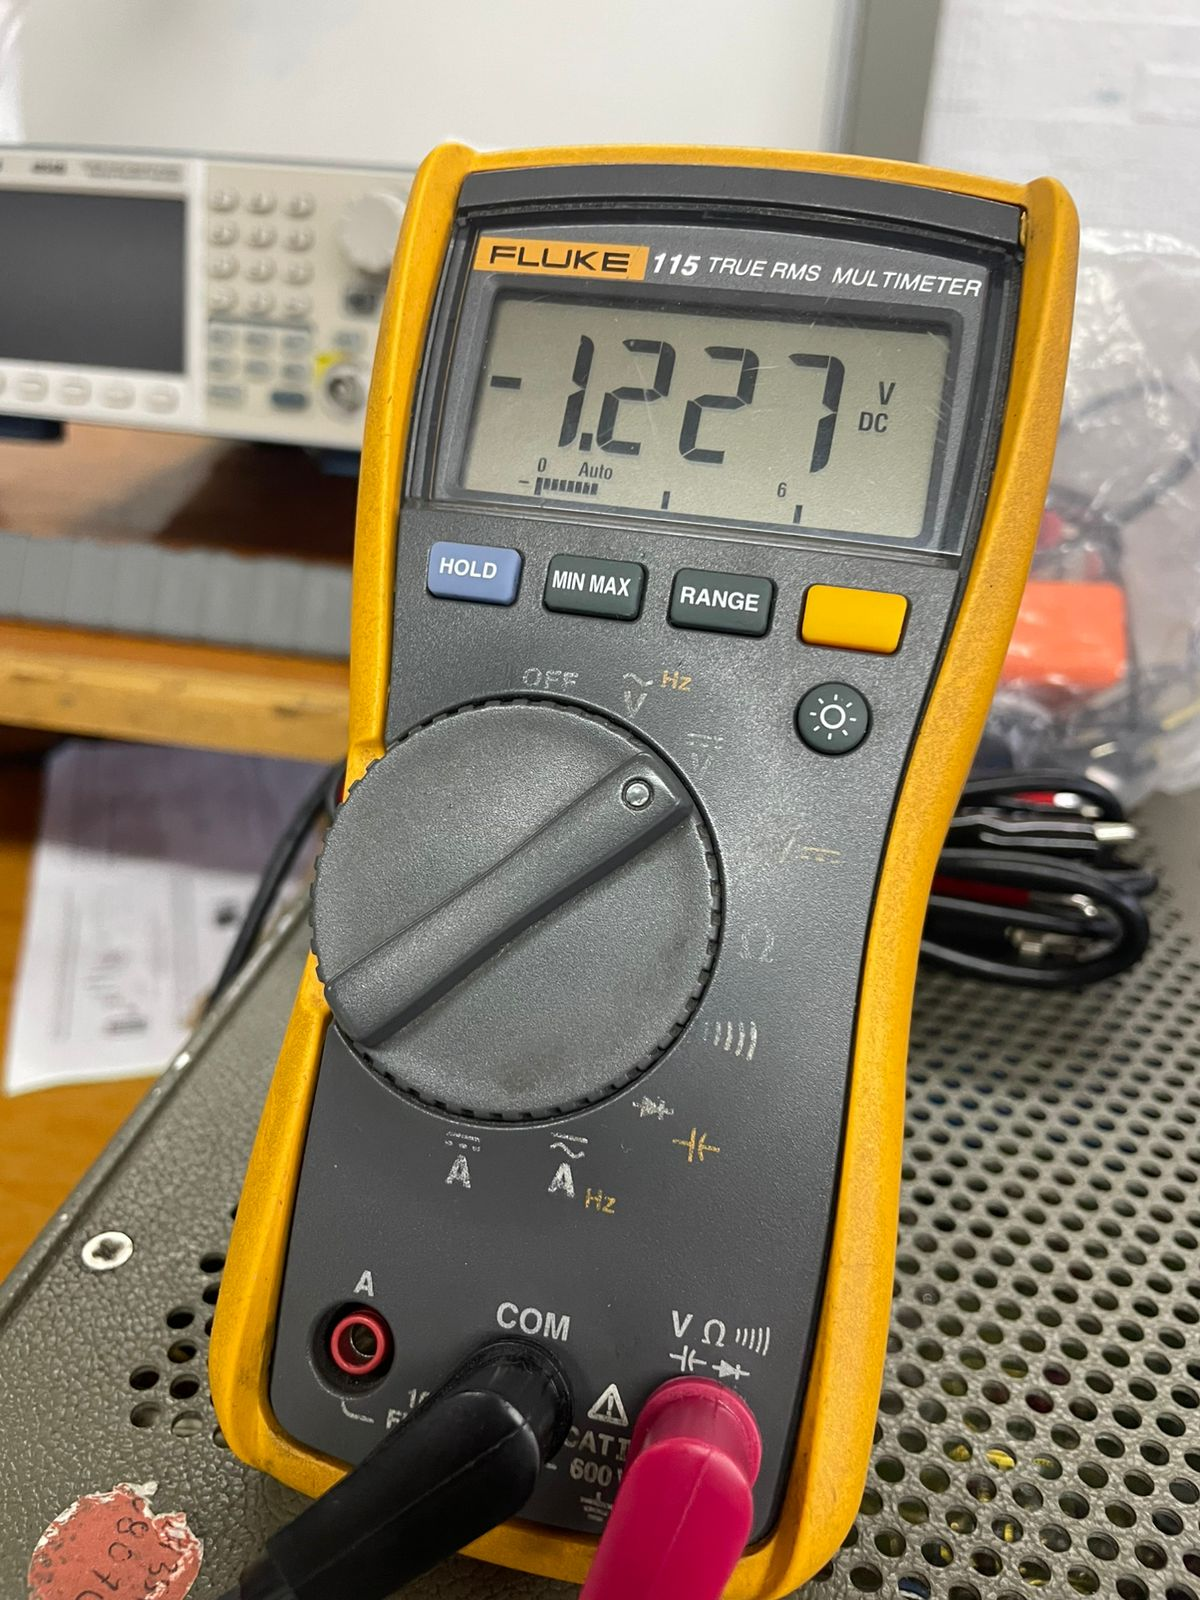
\includegraphics[width=0.8
			\linewidth]{assets/img/Tthevenin_medicion3_3.jpeg}
			\label{fig:thevenin_s6}
			\caption{Valor de la caída de voltaje para $R_{ab}=978 \Omega$..}
		\end{subfigure}
		\begin{subfigure}{0.3\textwidth}
		\centering
		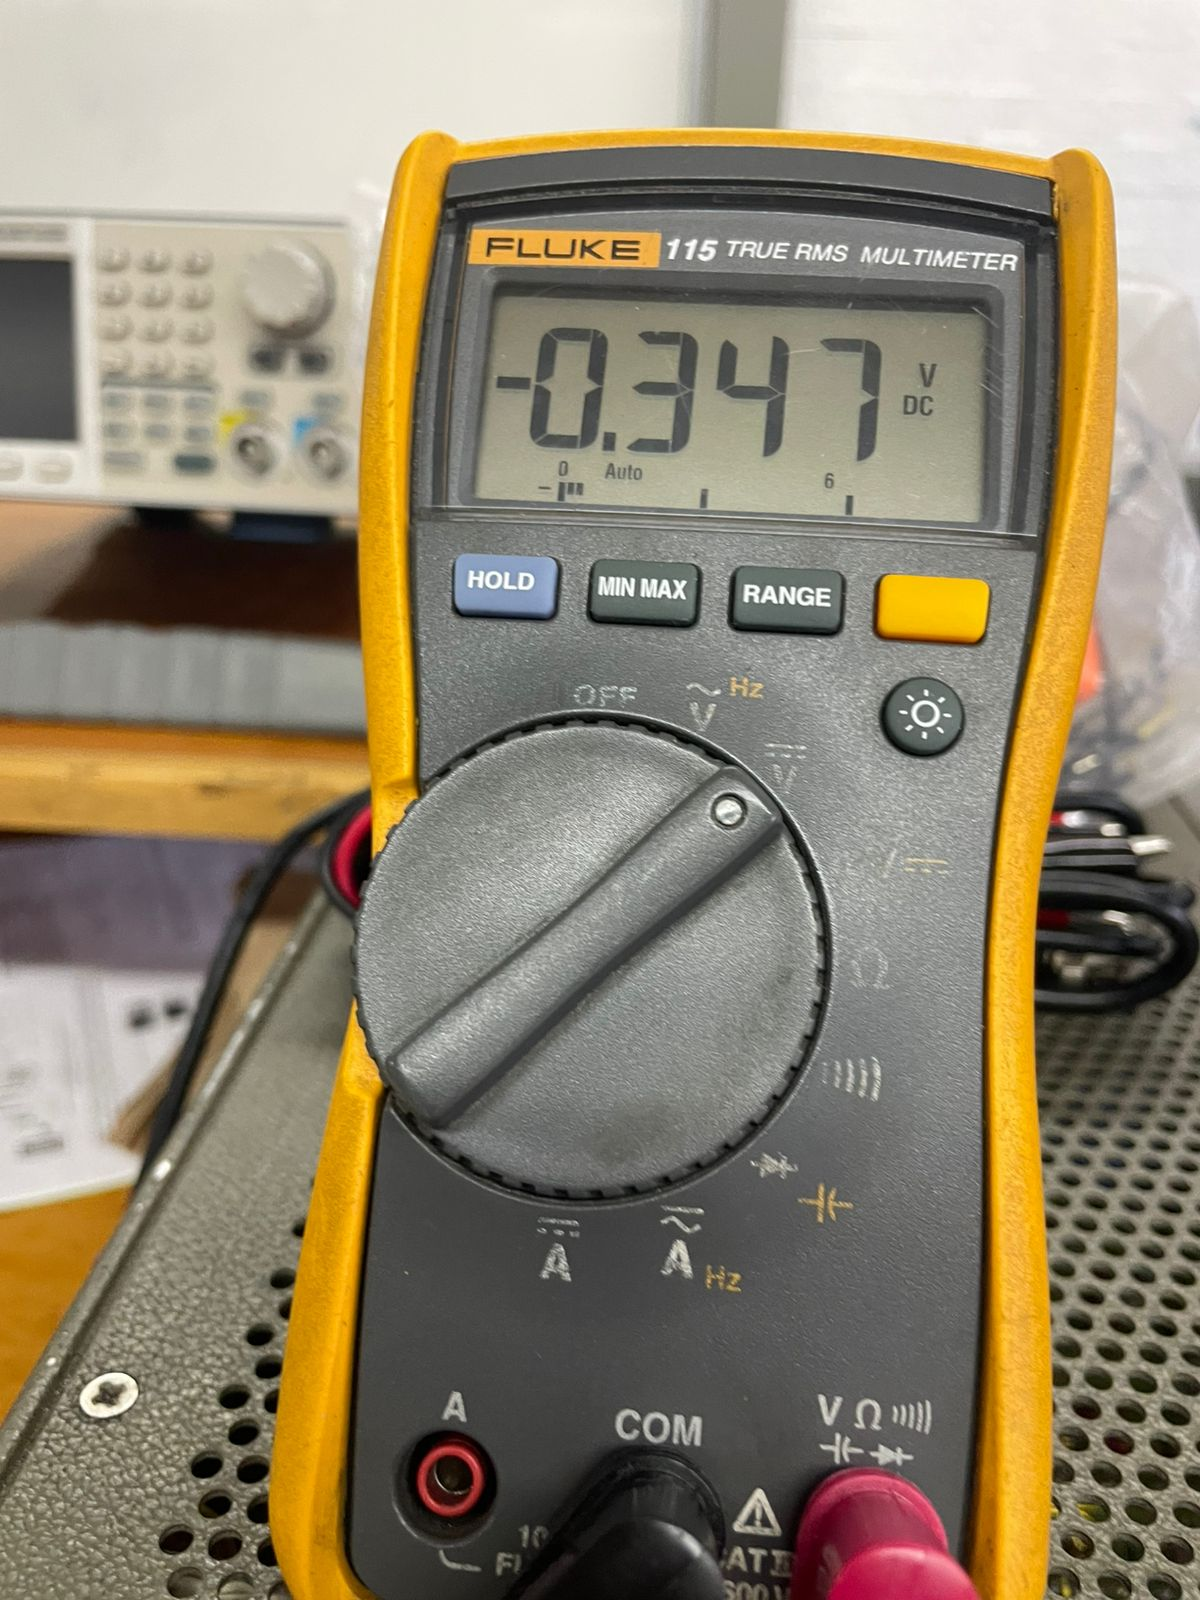
\includegraphics[width=0.8
		\linewidth]{assets/img/Tthevenin_medicion3_2.jpeg}
		\label{fig:thevenin_s7}
		\caption{Valor de la caída de voltaje para $R_{ab}=214 \Omega$.}
		\end{subfigure}			
	\end{figure}
	
	\begin{table}[H]
		\centering
		\caption{Comportamiento de la Red Original ante variaciones de carga.}
		\begin{tabular}{|l|c|c|c|}
			\hline
			\textbf{Parámetro} & \textbf{$R_{L1}$ ($9.88\text{ k}\Omega$)} & \textbf{$R_{L2}$ ($0.978\text{ k}\Omega$)} & \textbf{$R_{L3}$ ($214\text{ }\Omega$)} \\ \hline
			$V_{ab}$ [V] & -3.427 & -1.227 & -0.347 \\ \hline
			Potencia [mW] & 1.189 & 1.539 & 0.563 \\ \hline
		\end{tabular}
	\end{table}
	
	\item \textbf{Implementación del circuito equivalente:} Se armó un circuito compuesto por una fuente de voltaje y una resistencia en serie, calibradas lo más cerca posible a los valores de Thévenin obtenidos ($V' = -4.243 \text{ V}$ y $R' = 2.421 \text{ k}\Omega$). Se repitieron las mediciones con las mismas cargas para contrastar el comportamiento.
	
	\begin{figure}[H]
		\centering
		\begin{subfigure}{0.3\textwidth}
			\centering
			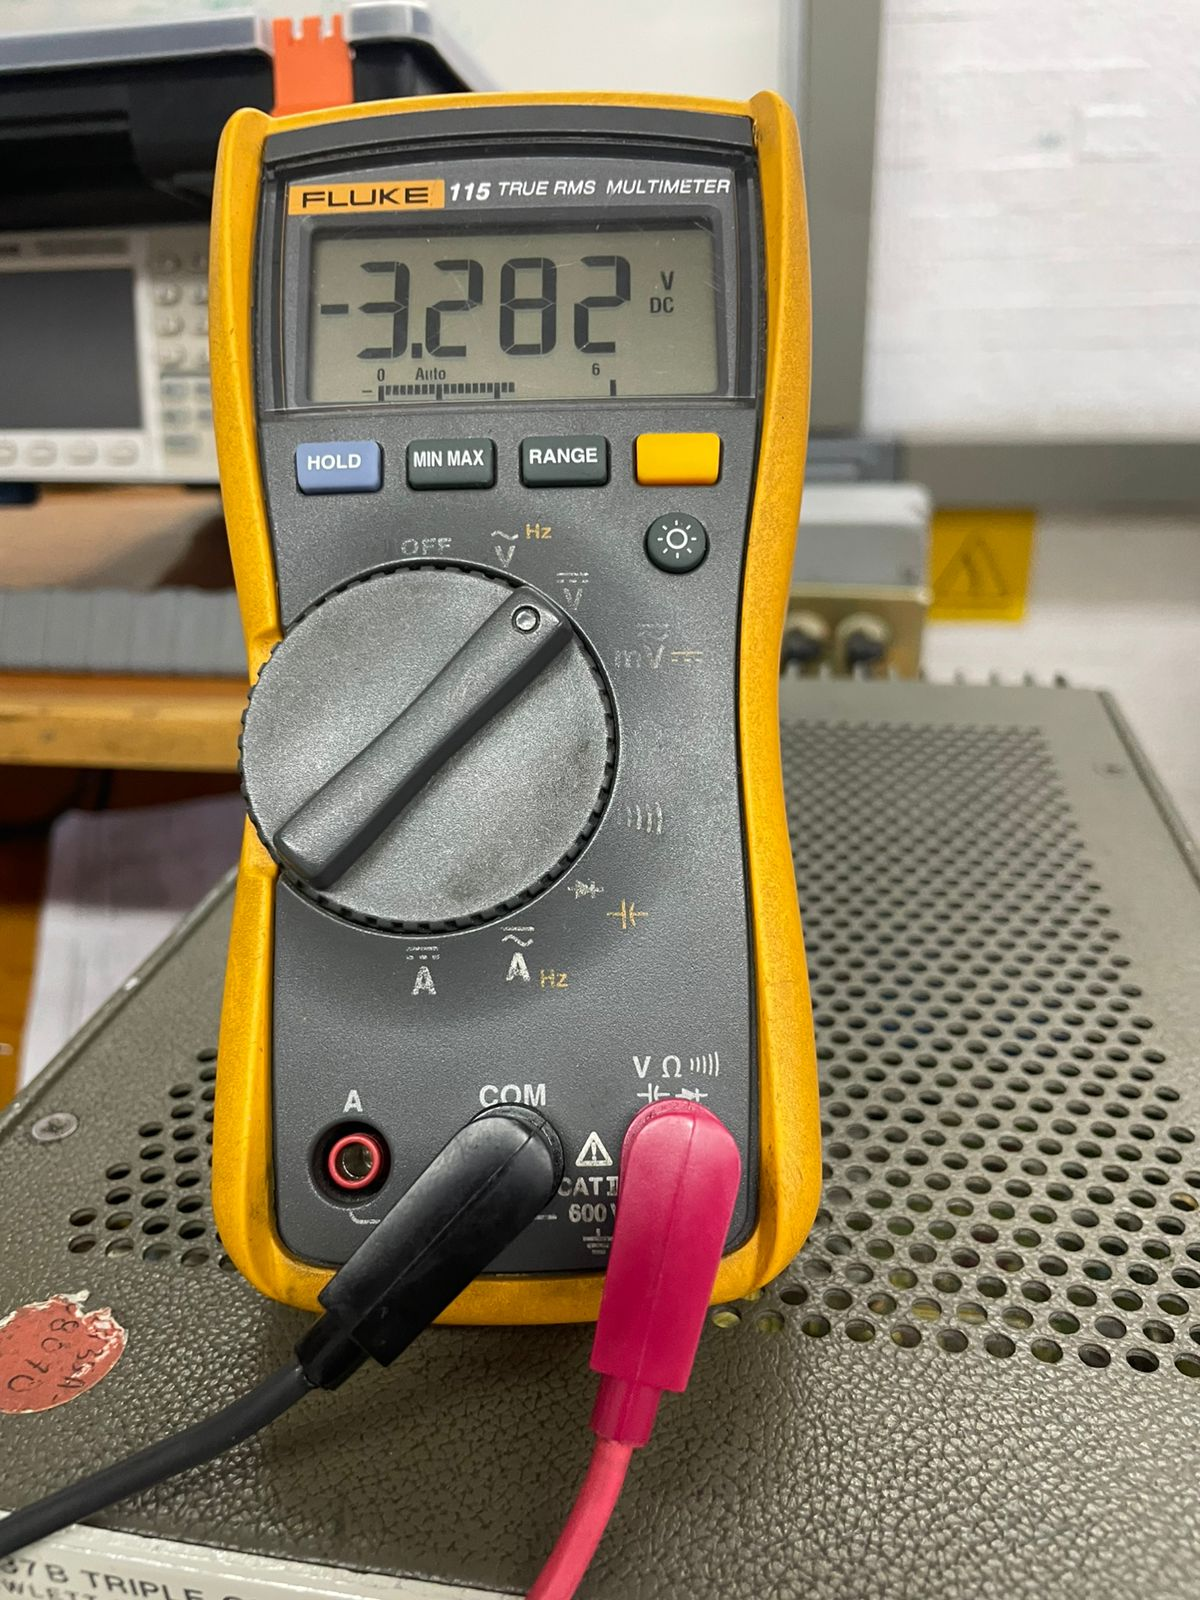
\includegraphics[width=0.8 \linewidth]{assets/img/Tthevenin_medicion4_1.jpeg}
			\label{fig:thevenin_s8}
			\caption{Valor de la caída de voltaje para $R_{ab}=9.88 \text{k}\Omega$.}
		\end{subfigure}
		\begin{subfigure}{0.3\textwidth}
			\centering
			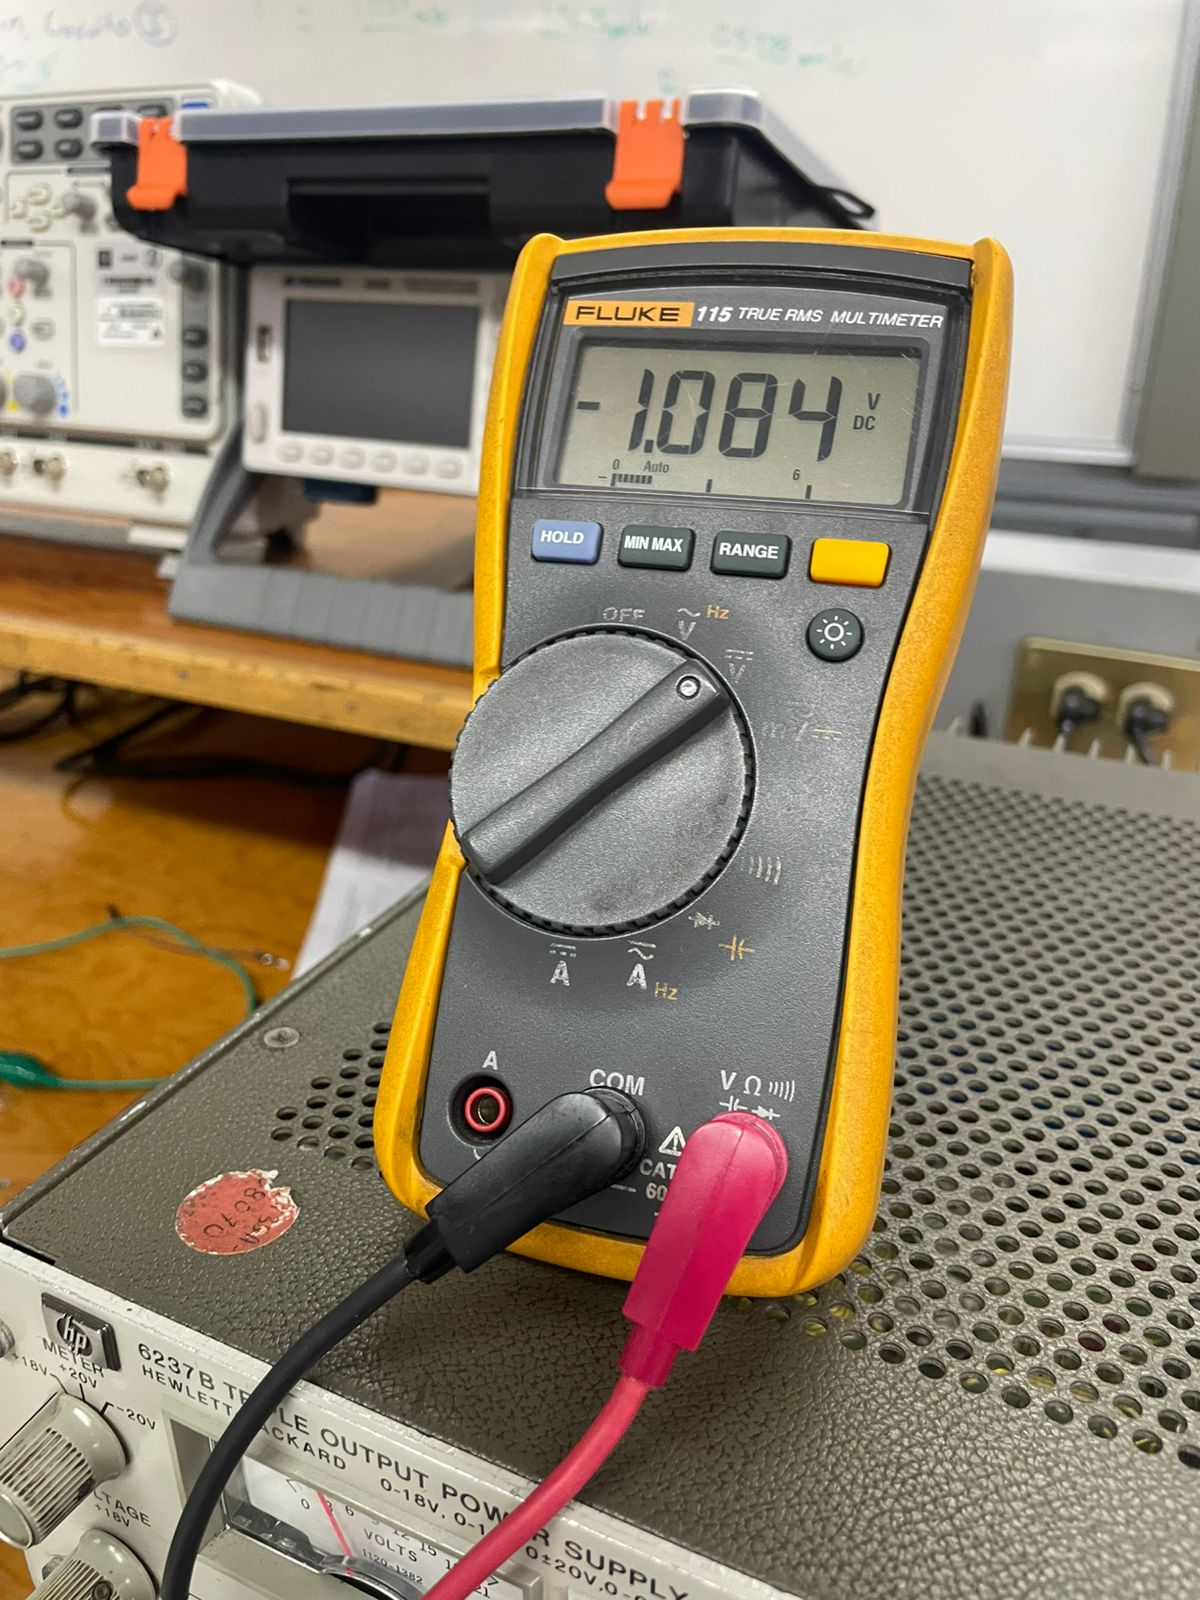
\includegraphics[width=0.8
			\linewidth]{assets/img/Tthevenin_medicion4_2.jpeg}
			\label{fig:thevenin_s9}
			\caption{Valor de la caída de voltaje para $R_{ab}=978 \Omega$..}
		\end{subfigure}
		\begin{subfigure}{0.3\textwidth}
			\centering
			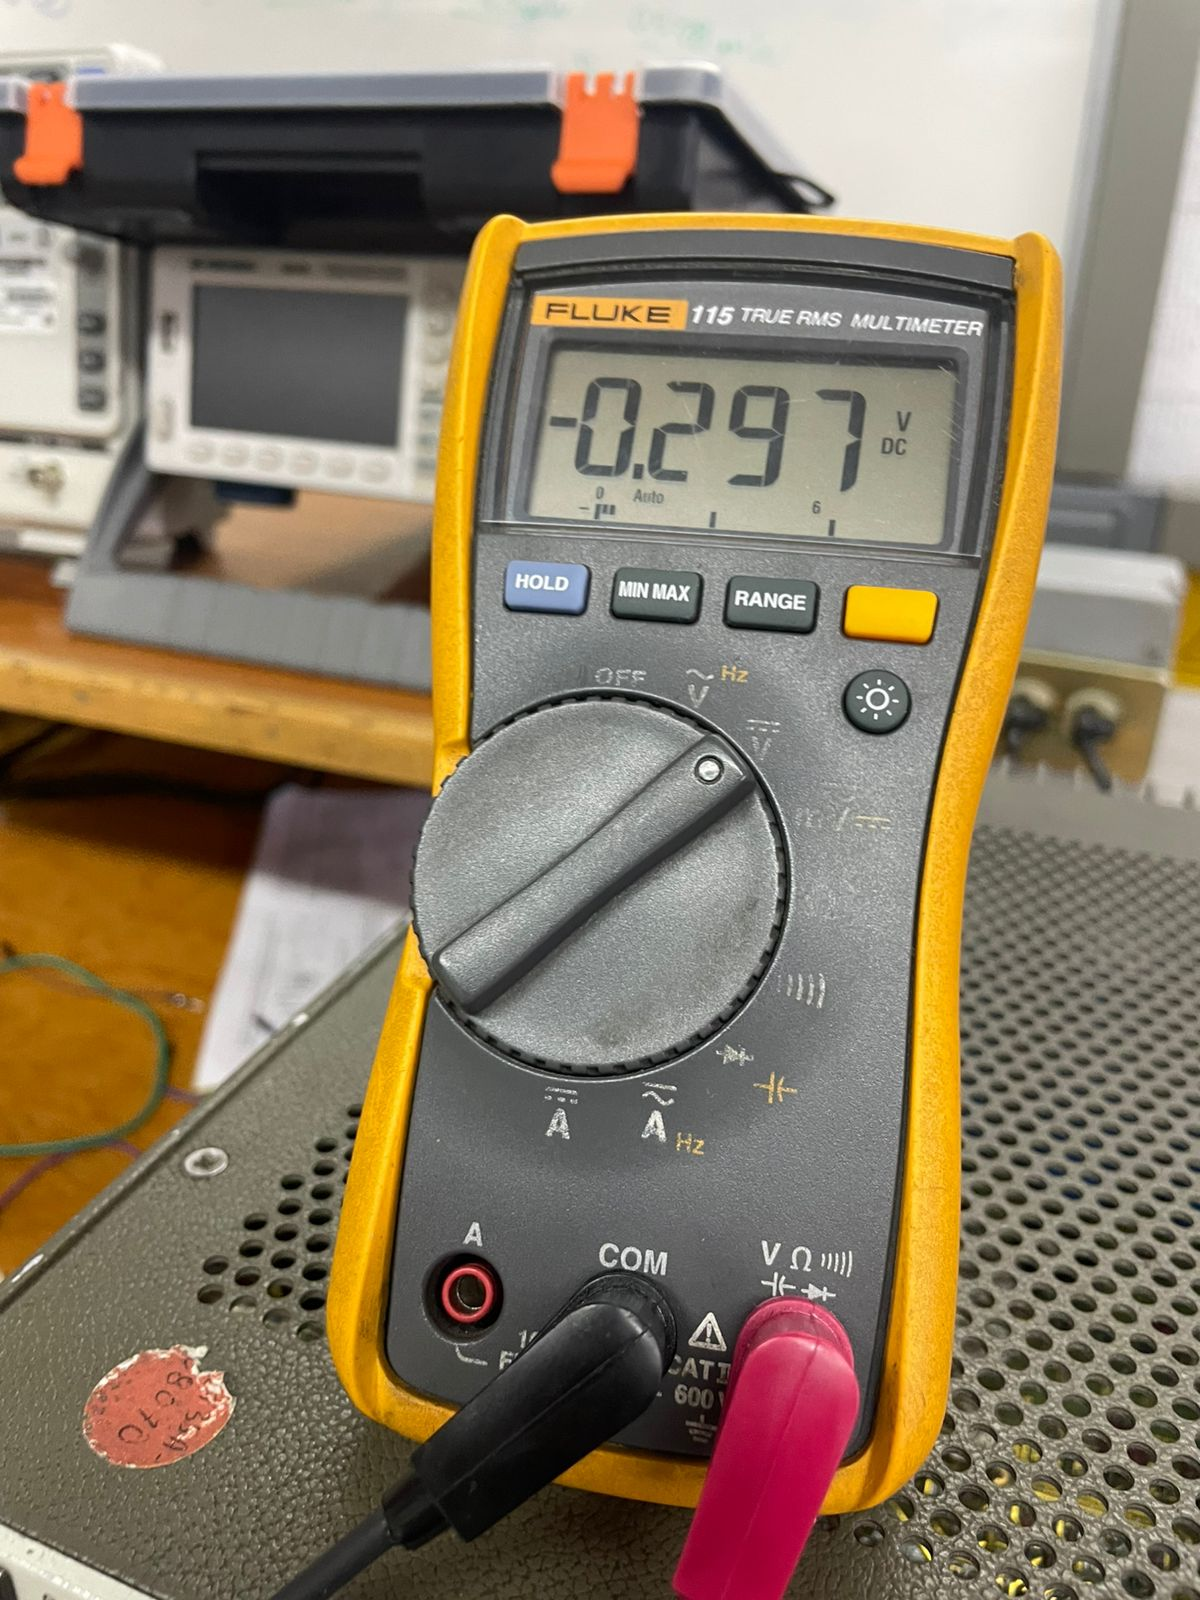
\includegraphics[width=0.8
			\linewidth]{assets/img/Tthevenin_medicion4_3.jpeg}
			\label{fig:thevenin_s10}
			\caption{Valor de la caída de voltaje para $R_{ab}=214 \Omega$.}
		\end{subfigure}			
	\end{figure}
	
\begin{table}[H]
	\centering
	\caption{Comportamiento del Circuito Equivalente ante variaciones de carga.}
	\begin{tabular}{|l|c|c|c|}
		\hline
		\textbf{Parámetro} & \textbf{$R_{L1}$ ($9.88\text{ k}\Omega$)} & \textbf{$R_{L2}$ ($0.978\text{ k}\Omega$)} & \textbf{$R_{L3}$ ($214\text{ }\Omega$)} \\ \hline
		$V_{ab}$ [V] & -3.281 & -1.081 & -0.297 \\ \hline
		Potencia [mW] & 1.089 & 1.195 & 0.412 \\ \hline
	\end{tabular}
\end{table}
	
\end{enumerate}


\textbf{Análisis de resultados}

Los datos obtenidos en las tablas comparativas demuestran la validez del Teorema de Thévenin, ya que el circuito equivalente replica con fidelidad la tendencia de respuesta de la red original ante variaciones de carga. En ambos sistemas, se observa que la tensión de salida $V_{ab}$ disminuye conforme la resistencia de carga $R_L$ se reduce, comportándose como un divisor de tensión dependiente de la impedancia de la red.

No obstante, se registra una discrepancia sistemática en los valores de tensión. Esta diferencia se atribuye primordialmente a las limitaciones técnicas en la calibración de las fuentes de laboratorio. El modelo equivalente se implementó con una tensión de $-4.243 \text{ V}$, valor ligeramente inferior a los $-4.26 \text{ V}$ de la red activa original. Asimismo, la resistencia de Thévenin empleada ($2.421 \text{ k}\Omega$) presentó una desviación respecto al valor experimental nominal ($2.424 \text{ k}\Omega$). Estas variaciones en los parámetros iniciales del equivalente explican por qué el error relativo se acentúa en la carga de $214 \text{ }\Omega$, donde la red es más sensible a las caídas de tensión internas.

Un hallazgo fundamental en este análisis es el comportamiento de la potencia disipada por la carga. De acuerdo con los datos experimentales, la potencia no sigue una relación lineal con la resistencia, sino que presenta un punto máximo. Se observa que la carga $R_{L2}$ ($0.978 \text{ k}\Omega$) registra la mayor transferencia de energía ($1.539 \text{ mW}$ en la red original), superando tanto a la carga de mayor valor como a la de menor valor. 

Este fenómeno valida de forma práctica el \textbf{Teorema de Máxima Transferencia de Potencia}, el cual dicta que la entrega de energía es óptima cuando $R_L$ se aproxima al valor de la resistencia de Thévenin ($R_{th} = 2.424 \text{ k}\Omega$). Dado que $R_{L2}$ es el valor más cercano al punto de acoplamiento de impedancias en comparación con los extremos de $9.88 \text{ k}\Omega$ y $214 \text{ }\Omega$, los resultados confirman que el circuito equivalente no solo modela correctamente las tensiones de la red, sino también su capacidad de suministro energético.

A pesar de las tolerancias de los componentes y las dificultades de calibración, se concluye que una red lineal activa compleja puede simplificarse a una sola rama equivalente. Esta representación permite predecir con precisión el comportamiento de una carga arbitraria y optimizar el rendimiento del sistema, simplificando significativamente el proceso de análisis y diseño en ingeniería.
\subsubsection{Parte teórica}

Para validar la precisión del modelo experimental y fundamentar la unicidad de la solución, se realizó una réplica del experimento en un entorno de simulación ideal. Este proceso permite contrastar los valores reales con una referencia teórica libre de las tolerancias físicas de los componentes.

\begin{enumerate}
	\item \textbf{Obtención de parámetros de Thévenin ideales:} Se simuló la red lineal activa original. Se midió la tensión de circuito abierto ($V_{th}$) y se determinó la resistencia equivalente ($R_{th}$) cortocircuitando las fuentes de alimentación ($E_1$ y $E_2$).
	
	\begin{figure}[H]
		\centering
		\begin{subfigure}{0.45\textwidth}
			\centering
			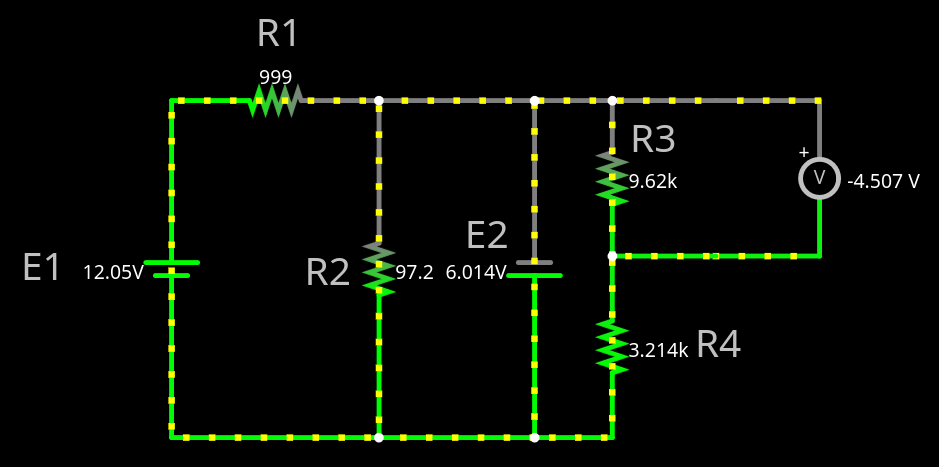
\includegraphics[width=0.8 \linewidth]{assets/img/Tthevenin_simulacionV.png}
			\label{fig:thevenin_s11}
			\caption{Obtención de $V'$.}
		\end{subfigure}
		\begin{subfigure}{0.45\textwidth}
			\centering
			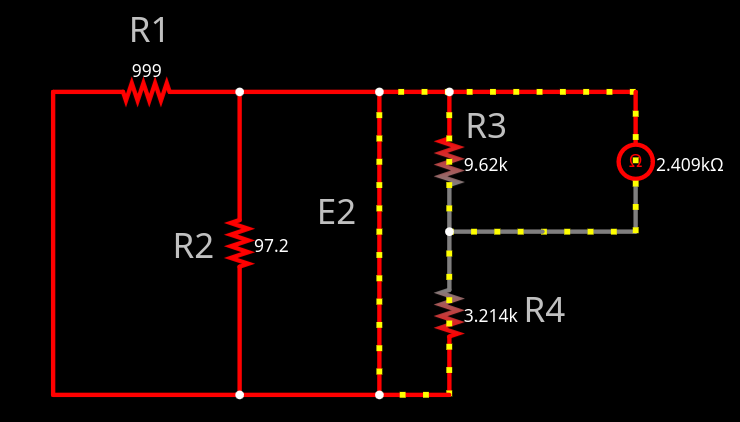
\includegraphics[width=0.8
			\linewidth]{assets/img/Tthevenin_simulacionR.png}
			\label{fig:thevenin_12}
			\caption{Obtención de $R'$.}
		\end{subfigure}			
	\end{figure}
	
	\begin{itemize}
		\item Voltaje de Thévenin ideal ($V_{th}$) = $-4.507 \text{ V}$
		\item Resistencia de Thévenin ideal ($R_{th}$) = $2.409 \text{ k}\Omega$
	\end{itemize}
	
	\item \textbf{Prueba de la red activa original (Simulación):} Se conectaron las tres resistencias de carga ($R_L$) en la red compleja para obtener los valores de referencia de voltaje y potencia.
	
	\begin{figure}[H]
		\centering
		\begin{subfigure}{0.3\textwidth}
			\centering
			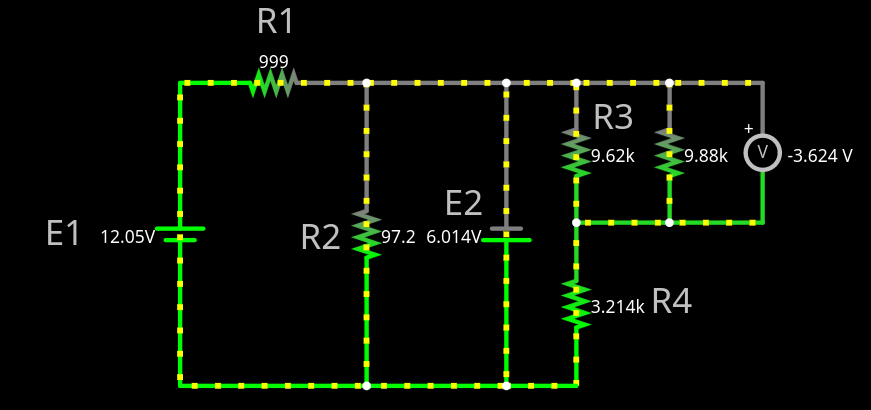
\includegraphics[width=0.8 \linewidth]{assets/img/Tthevenin_medicionS1.png}
			\label{fig:thevenin_s12}
		\end{subfigure}
		\begin{subfigure}{0.3\textwidth}
			\centering
			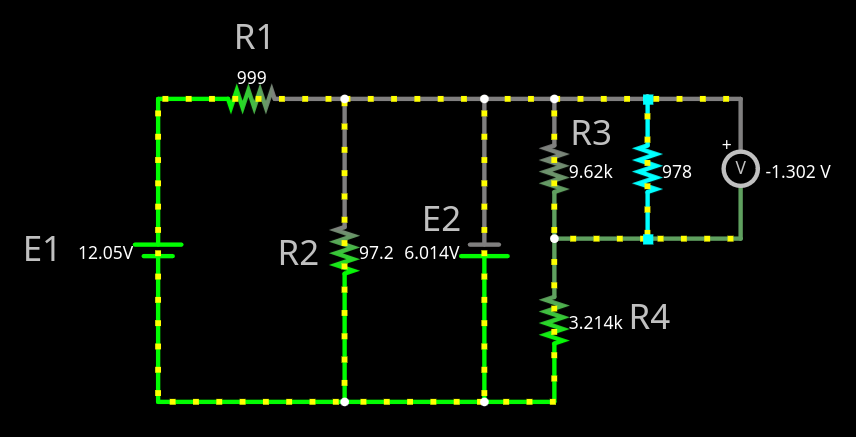
\includegraphics[width=0.8
			\linewidth]{assets/img/Tthevenin_medicionS2.png}
			\label{fig:thevenin_s13}
		\end{subfigure}
		\begin{subfigure}{0.3\textwidth}
			\centering
			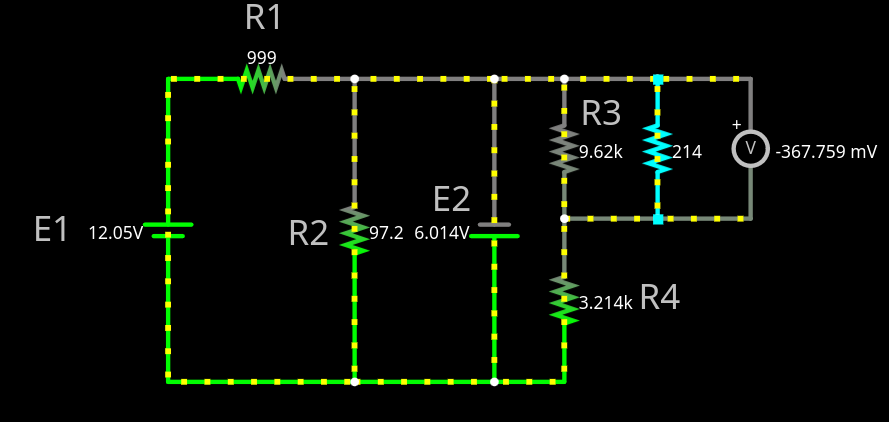
\includegraphics[width=0.8
			\linewidth]{assets/img/Tthevenin_medicionS3.png}
			\label{fig:thevenin_s14}
		\end{subfigure}			
	\end{figure}
	
	\begin{table}[H]
		\centering
		\caption{Simulación: Comportamiento de la Red Original ante variaciones de carga.}
		\begin{tabular}{|l|c|c|c|}
			\hline
			\textbf{Parámetro} & \textbf{$R_{L1}$ ($9.88\text{ k}\Omega$)} & \textbf{$R_{L2}$ ($0.978\text{ k}\Omega$)} & \textbf{$R_{L3}$ ($214\text{ }\Omega$)} \\ \hline
			$V_{ab}$ [V] & -3.624 & -1.302 & -0.368 \\ \hline
			Potencia [mW] & 1.329 & 1.733 & 0.632 \\ \hline
		\end{tabular}
	\end{table}
	

	\item \textbf{Implementación del circuito equivalente (Simulación):} Se construyó el modelo simplificado utilizando una fuente ideal de $-4.507 \text{ V}$ y una resistencia de $2.409 \text{ k}\Omega$.
	
	
	\begin{figure}[H]
		\centering
		\begin{subfigure}{0.3\textwidth}
			\centering
			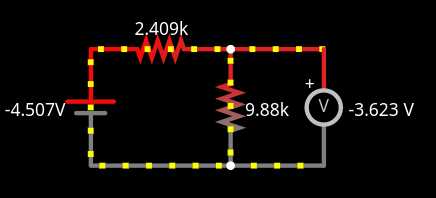
\includegraphics[width=0.8 \linewidth]{assets/img/Tthevenin_medicionS4.png}
			\label{fig:thevenin_s15}
		\end{subfigure}
		\begin{subfigure}{0.3\textwidth}
			\centering
			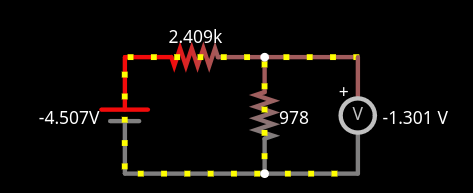
\includegraphics[width=0.8
			\linewidth]{assets/img/Tthevenin_medicionS5.png}
			\label{fig:thevenin_s16}
		\end{subfigure}
		\begin{subfigure}{0.3\textwidth}
			\centering
			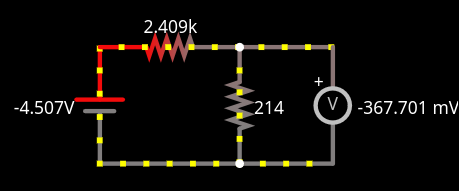
\includegraphics[width=0.8
			\linewidth]{assets/img/Tthevenin_medicionS6.png}
			\label{fig:thevenin_s17}
		\end{subfigure}			
	\end{figure}
	
	\begin{table}[H]
		\centering
		\caption{Simulación: Comportamiento del Circuito Equivalente ante variaciones de carga.}
		\begin{tabular}{|l|c|c|c|}
			\hline
			\textbf{Parámetro} & \textbf{$R_{L1}$ ($9.88\text{ k}\Omega$)} & \textbf{$R_{L2}$ ($0.978\text{ k}\Omega$)} & \textbf{$R_{L3}$ ($214\text{ }\Omega$)} \\ \hline
			$V_{ab}$ [V] & -3.623 & -1.301 & -0.368 \\ \hline
			Potencia [mW] & 1.328 & 1.731 & 0.632 \\ \hline
		\end{tabular}
	\end{table}
	
\end{enumerate}

\textbf{Análisis de resultados}

Al contrastar los datos teóricos con los experimentales, se observa que la simulación arroja una equivalencia casi absoluta (error < 0.1\%) entre la red original y su equivalente de Thévenin. Esto confirma que el modelo de dos terminales es una representación matemática exacta de la red activa.La diferencia de aproximadamente $0.24 \text{ V}$ entre la tensión de Thévenin ideal ($-4.507 \text{ V}$) y la experimental ($-4.26 \text{ V}$) se explica por la resistencia interna de las fuentes de laboratorio y la impedancia de los cables, factores que no se consideran en el entorno de simulación. No obstante, en ambos casos se verifica que la carga de $978 \text{ }\Omega$ es la que disipa la mayor cantidad de potencia al ser el valor más próximo a la resistencia de Thévenin ($2.4 \text{ k}\Omega$), validando nuevamente el teorema de máxima transferencia de potencia de forma universal.